\section{Middlebox Implementation}
\label{sec:netshaper-middlebox-implementation}

While it is possible to apply NetShaper framework's approach at any network layer, we chose to develop the system as an L4 (Transport Layer) proxy.
This enables the system to be easily deployable, entirely in userspace and without requiring any superuser privileges. 
Developing NetShaper at L2 (Data Link Layer) or L3 (Network Layer) would require the deployer to either have the ability to modify the OS kernel or deploy some form of kernel bypass.

\begin{figure}[!htb]
    \centering
    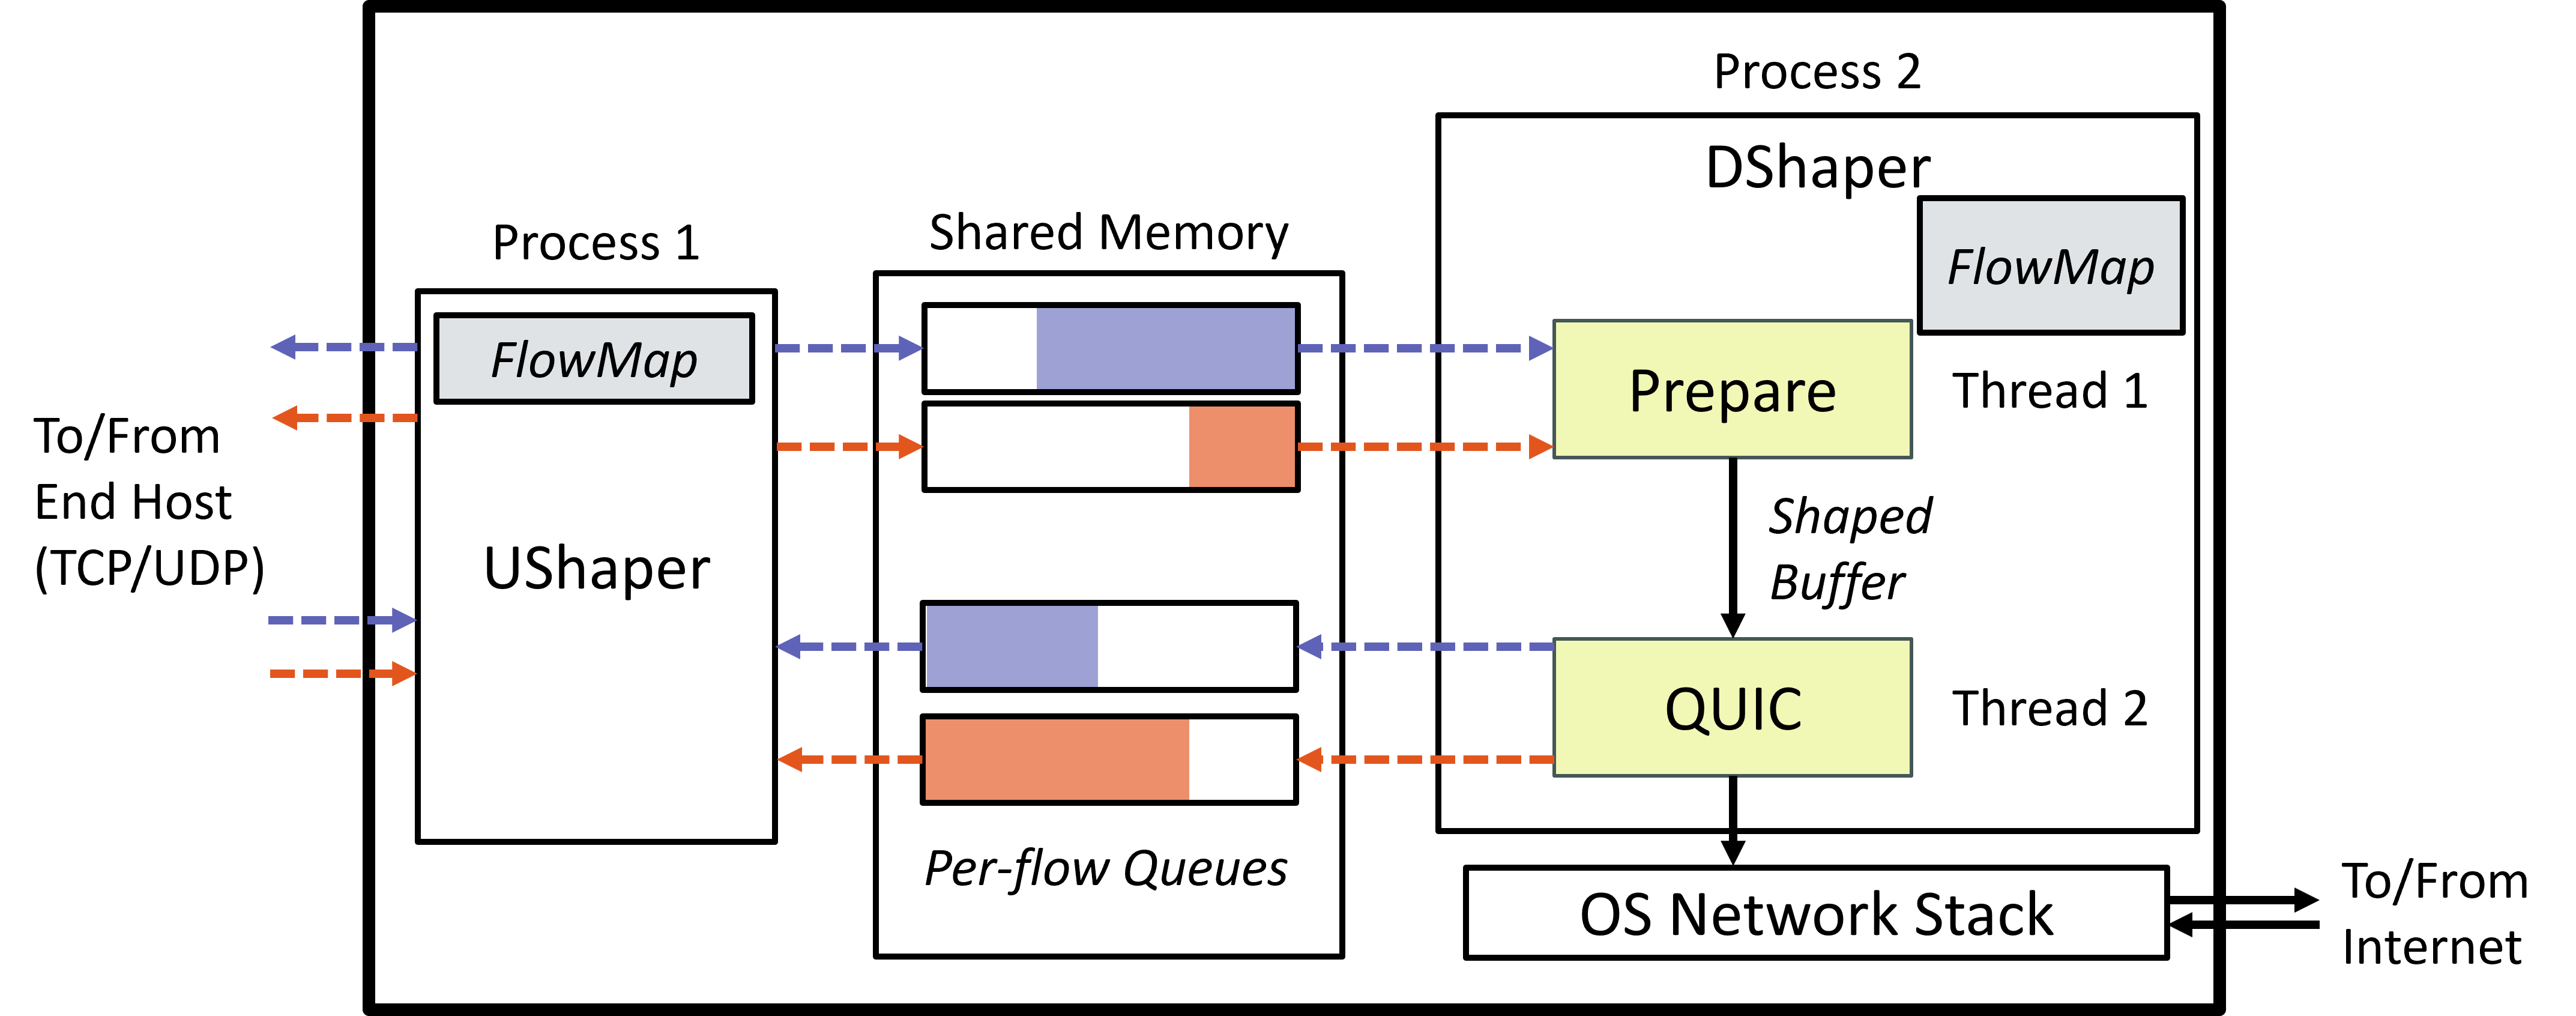
\includegraphics[width=\columnwidth]{figures/netshaper/middlebox-implementation.png}
    \caption{NetShaper Middlebox Implementation}
    \label{fig:middlebox-implementation}
\end{figure}

As outlined in \Cref{fig:middlebox-implementation}, NetShaper's middlebox consists of two main processes: \textit{UShaper} and \textit{DShaper}, and a shared memory between them.

\paragraph{Shared Memory.}
Both \textit{UShaper} and \textit{DShaper} have a shared memory between them.
The shared memory consists of $2*(k + 2)$ Lamport Queues (LQs) \cite{lamportqueue}
\footnote{Lamport Queues are lock-free single producer single consumer (SPSC) queues. They are useful to ensure that no locking is required when putting data in or pulling data out from the queues.}, 
where $k$ is the fixed number of \textit{data streams} that were configured at initialisation.
There is one queue for each direction of transmission for each of the $k$ streams that are initialised, and one for each of the \textit{control stream} and \textit{dummy stream}.

Similar to the stream types outlined in \Cref{sec:netshaper-designing-traffic-shaping-tunnel}, the \textit{control LQ} transmits the information about a connection establishment or termination by an end host application. 
The \textit{dummy LQ} carries dummy data that is received from or sent to the tunnel.
Each \textit{data LQ} carries the application byte stream that has been received from or has to be sent to the remote application.


\paragraph{UShaper.}
The \textit{UShaper} implements a client or a server to communicate with the end host.
The \textit{UShaper} also consists of a FlowMap 
\footnote{The NetShaper paper shows a shared FlowMap between the \textit{UShaper} and \textit{DShaper}. However, to avoid locking and signalling across processes, we improved the implementation to instead synchronise the FlowMap by using a \textit{control LQ} that is shared between the processes.}
that maps an end-host application with a corresponding pair of LQs.
\textit{UShaper} updates the FlowMap whenever an end-host application establishes or terminates a connection, and a \textit{control} message is generated and either sent or received on the \textit{control} LQ.
In addition, it assigns an unused pair of LQs (one outbound and one inbound) to a new client and revokes that whenever the client terminates the connection.
The \textit{UShaper} receives outbound traffic from the end host and enqueues the payload in the assigned LQ.
Similarly, it dequeues inbound traffic from the inbound LQs and sends it to the corresponding end hosts.
% We have implemented \textit{UShaper} in 1100 lines of C++ code.

\paragraph{DShaper.}
The \textit{DShaper} consists of two threads, \textit{Prepare} and \textit{QUIC worker}, and a FlowMap.
The FlowMap maps an LQ with a pre-initialised QUIC stream.
The \textit{Prepare} thread measures the data available in the outbound LQs at the start of the window $W$.
It then adds noise to this available size based on the DP parameters.
Finally, it enqueues the payload and padding that needs to be transmitted.
The \textit{QUIC worker} transmits the enqueued data out to the network.
It also processes the received data, places it in the relevant LQ, and updates the FlowMap when necessary.
% We have implemented \textit{DShaper} in 1800 lines of C++ code
% \footnote{\label{footnote:msquic-loc} Both \textit{UShaper} and \textit{DShaper} consist of the MSQUIC implementation of QUIC, which is 180k lines of code, and is a part of NetShaper's TCB.}.

\subsection{Ensuring secret-independent shaping}
\label{subsec:netshaper-secret-independent-shaping-implementation}

To enforce DP guarantees, \textit{DShaper} needs to transmit $L + \eta$ bytes in every finite interval $W$.
To achieve this, \textit{DShaper} should satisfy the following properties.
\textbf{P1}: The \textit{Prepare} thread should calculate $L + \eta$, prepare a buffer of that size, and enqueue that buffer for the \textit{QUIC worker} thread to transmit within $W$.
\textbf{P2}: The \textit{QUIC worker} thread should encrypt the packets from the buffer and forward them to the UDP stack, such that the total size of the payload prepared in $W$ is $L + \eta$.
\textbf{P3}: The UDP stack should transmit the encrypted packets within $W$.
Thanks to the post-processing property of DP, it suffices to only ensure P1, and \textbf{P4.} that the \textit{QUIC worker} thread prepares the QUIC packets independently of the secret data.

However, there are some challenges in satisfying P1 and P4.
As both the \textit{Prepare} thread and \textit{UShaper} deal with secret-dependent data, their execution time may affect the observable network behaviour, which in turn may lead to exposed secrets.
While the end host application is isolated from the middlebox, its flow control may be secret dependent and can affect the execution time of the \textit{Prepare} thread.
For example, the presence or absence of an application's traffic can affect the time it takes for the \textit{Prepare} thread to prepare the buffers.
If the \textit{QUIC worker} thread starts transmitting immediately, the secret dependent information may be visible in the network behaviour. 
This would also break P4, as the \textit{QUIC worker} thread prepares the QUIC packets based on the secret-dependent flow control.
NetShaper addresses this by ensuring that the \textit{Prepare} thread takes a fixed amount of time ($T_{prep}$) to prepare the shaped buffer.
Also, it locks the buffer when enqueuing it to the \textit{QUIC worker} so that the \textit{QUIC worker} does not start preparing the packets and transmitting them immediately.
The \textit{Prepare} thread releases the lock after a fixed amount of time $T_{enq}$.
As such, the \textit{QUIC worker} thread only receives the shaped buffer at regular intervals of time.
We empirically profile the time taken by the \textit{Prepare} thread for $T_{prep}$ and $T_{enq}$ for buffers of various lengths and set the values to the maximum observed, with an additional margin on top.
We have outlined pseudo-code for both the \textit{Prepare} thread and the \textit{QUIC worker} thread in \Cref{lst:prepare_and_worker}.


To ensure further isolation, the \textit{Prepare} and \textit{QUIC worker} threads are both run on separate physical cores.
\textit{UShaper} runs on a yet different core to ensure that the sending and receiving of unshaped, secret-dependent data does not affect the execution time of either of the \textit{DShaper} threads.
We assume that QUIC's encryption and decryption time correlates only with the shaped buffer's size, not its content.



\begin{minipage}{\textwidth}
\lstinputlisting[language=Python]{code/netshaper/prepare_and_worker.py}
\captionsetup{type=lstlisting}
\caption{Pseudo-code of the \textit{Prepare} and \textit{QUIC Worker} threads}
\label{lst:prepare_and_worker}
\end{minipage}
